\chapter{Pruebas y resultados}

En este capítulo del Trabajo se realizará un análisis de la fase final del proyecto, en la que, una vez finalizada la programación y la instalación de los dispositivos en la vivienda, se hará un examen exhaustivo al comportamiento de todos los mecanismos y la relación entre ellos,  comprobando la robustez del diseño y subsanando pequeños bugs o fallos no identificados en las fases anteriores, así como el funcionamiento adecuado de los equipos y mecanismos que lo componen.

\section{Puesta en marcha}
En esta sección se describirá en detalle la fase final del proyecto, consistente en que, una vez finalizada la instalación física de los componentes en la vivienda, se realizarán una serie de pruebas y comprobaciones para confirmar que tanto la programación como su volcado en los mecanismos han sido correctos, sin llegar a suceder o sin alcanzar algún estado inesperado o incorrecto que hiciese detenerse o incluso fallar el sistema completo. Con estas pruebas también se detectan fallos cometidos durante la fase de instalación del sistema eléctrico como cables mal etiquetados que dan lugar a confusiones y comportamientos anómalos de los mecanismos, o incluso derivaciones y otra serie de cuestiones relacionadas con el cableado y su acometida eléctrica. Todas estas pruebas, chequeos y correcciones se engloban en el término Puesta en Marcha.\\\\

Por motivos de tiempo, las primeras pruebas que se han realizado sobre los equipos son las relacionadas con los módulos lógicos implementados en el X1. Esto es debido a que en caso de no comportarse de manera idéntica en la instalación que en las simulaciones y pruebas en el ordenador, ya sea por contener programación incorrecta o por la influencia de otras variables del sistema no contempladas durante estas simulaciones, su modificación y posterior fase de pruebas y simulaciones tendría un gran coste en términos de tiempo, lo que finalmente se traduce en una pérdida del beneficio y del margen de ganancia que obtendría la empresa, alejándolo por tanto de su objetivo final.\\\\

Debido a este requerimiento de enviar a una persona a realizar pruebas sobre la propia instalación real, las simulaciones y pruebas en el ordenador toman una gran relevancia a la hora de no invertir o gastar recursos y tiempo que podrían restar valor final al total del proyecto. Por lo tanto, utilizando el software \textit{Gira Project Assistant}, se han testeado y comprobado encarecidamente las programaciones lógicas desarrolladas antes de realizar la prueba definitiva en la vivienda.\\\\

Una vez finalizada esta parte de la Puesta en Marcha, se continuará volcando la programación completa a todos los módulos y mecanismos que componen el sistema, permitiendo así realizar el resto de comprobaciones. Estas rutinas de chequeo han sido diseñadas y plasmadas en un documento (confidencial) por el propio ingeniero que ha diseñado el proyecto y posteriormente, ampliadas por expertos con mayor experiencia y conciencia de los fallos más habituales y también los más perjudiciales. Esta combinación permite buscar y encontrar con una mayor precisión y rapidez los errores cometidos a cualquier persona con cualificación y conocimientos en la materia, logrando así no copar el tiempo al completo del diseñador y programador. \\

Cuando todos los mecanismos hayan recibido su programación, se comenzará realizando las pruebas más simples, rápidas y sencillas como el ON/OFF de la las luminarias o la subida y bajada de las persianas, e irá incrementando su complejidad hasta finalmente realizar un chequeo completo del sistema de climatización teniendo en cuenta todas las posibilidades de combinaciones y comportamientos posibles que este sistema puede llegar a alcanzar. \\\\
Una vez se han validado todas las pruebas y especificaciones recogidas en el documento anteriormente mencionado, se realizará una demostración al cliente, explicando a su vez el funcionamiento final que tendrá el sistema instalado en su vivienda, validando de esta manera la consecución de los requisitos iniciales planteados y dando por finalizando así la Puesta en Marcha, y por tanto, el proyecto.
\vspace{2cm}

\section{Resultados}

Como se comentaba en el apartado anterior, las primeras pruebas se realizan sobre los módulos lógicos implementados en el X1 en la misma consola de simulación del software de programación. Esta simulación permite asignar un valor inicial a cada entrada que contenga el módulo lógico, y posteriormente su modificación y visualización con la capacidad de controlar la velocidad de reproducción, llegando incluso a permitir su simulación por pasos. Todo ello permitirá al programador realizar un exhaustivo estudio del comportamiento del módulo diseñado, permitiendo así la validación del mismo. Por tanto, haciendo uso de esta herramienta, se confirmó el correcto funcionamiento de las programaciones lógicas a implementar.\\\\
Una vez completada esta fase, se comienza con la etapa de volcado de la programación sobre los elementos ya instalados en la vivienda, con la intención de verificar el correcto funcionamiento y realizar una prueba de validación con el cliente, explicando a la vez su funcionamiento y manejo. Durante esta fase, se hace notorio el funcionamiento irregular de la regulación de la las luminarias, no comportándose los mecanismos instalados tal y como se esperaba: debido a la alta frecuencia de ocupación del bus que requiere el módulo lógico, muchos de los telegramas se extravían y provocan que las luces no reaccionen o incluso titilen, sobrecalentando al módulo X1. \\\\
Debido a la aparición de este comportamiento, se hace necesario el replanteo de la estructura del módulo lógico para lograr una mejora notable en su funcionamiento, que será descrita en el siguiente apartado (\ref{sec:mejoras}). Durante el resto del volcado de la programación y de las pruebas de funcionamiento no se encontraron mayores problemas que aquellos relacionados con confusiones en el cableado de los elementos hasta el cuadro, que fueron subsanadas rápidamente e insitu gracias a la participación de los técnicos de instalación.

\vspace{2cm}

\section{Mejoras}
\label{sec:mejoras}

Como ya se comentó en capítulos anteriores, una vez iniciada la puesta en marcha, es necesaria la aplicación de ciertas mejoras para optimizar el funcionamiento de nuestra instalación, como es el caso del bloque lógico encargado de la regulación de las luminarias. Este bloque sufrirá modificaciones desde la base de su concepción, por lo que se procederá a realizar un análisis del nuevo modo de programación con el que serán controladas esta clase de luces.\\\\
En primer lugar, las teclas de los pulsadores cambian la programación de su funcionalidad del tipo conmutación al de regulación con repetición de telegrama, en el que su tecla izquierda tendrá asignada la acción de desconexión, mientras que por el contrario, la derecha tendrá de conexión. Los intervalos de regulación se fijan en 12,5\% como reacción ante la pulsación larga. Con estos dos ajustes se logra obtener el siguiente patrón de comportamiento en el envío de los telegramas hacia la misma dirección de grupo:

\begin{flushleft}
\begin{table}[H]
\centering
\resizebox{10cm}{!} {
\begin{tabular}{|c|c|c|}
\hline
\backslashbox{Tecla}{Valor} & Pulsacion corta & Pulsacion larga \\ \hline 
\rule[0mm]{0mm}{4mm}
Izquierda & 0 & 12 \\ \hline
\rule[0mm]{0mm}{4mm}
Derecha &1 & -12\\ \hline
\end{tabular}
}
\caption{Valores enviados a través de los pulsadores}
\end{table}
\end{flushleft}

Una vez definidos los valores que se generarán al actuar sobre las teclas de los pulsadores, se crea un módulo lógico que, en cuanto a la funcionalidad ON/OFF, permite ejercer una acción de conmutación. Debido a que en la pulsación corta cada tecla envía siempre el mismo valor (0 ó 1) sobre la dirección de grupo \textit{Corta Pulsador X}(siendo X la dirección del pulsador a controlar), se crea la necesidad de que el sistema recuerde en qué valor se encontraba la luz anteriormente, entendiendo cualquier porcentaje de intensidad distinto de cero como ON, permitiendo así cambiar al estado contrario tras cada pulsación. \\
Por lo tanto, cada vez que por esa dirección de grupo se reciba un valor, este se hará pasar por dos módulos de Bloqueo. Cada uno de estos bloques únicamente permitirá el paso de uno de los dos valores, permaneciendo inactivo uno de ellos cuando el otro se encuentra activo, en función del valor que tome esa dirección de grupo; ya que, como ya se comentó en la sección de programación (Capítulo \ref{sec:prog}), estos bloques solo permiten el envío del valor recibido por su puerto “Entrada” si recibe un 0 en su puerto “Activo”. Para lograr esto, uno de los módulos de Bloqueo tendrá previo a su puerto “Activo” un inversor, haciendo así que se desbloquee ante la entrada de valor 0. Con el fin de enviar el último valor recibido, los puertos “Entrada” de los módulos de Bloqueo vendrán precedidos de bloques “Retardador de telegramas”, que retrasarán la lectura de este valor un segundo respecto a los del puerto “Activo”. Por otro lado, y de manera independiente, se leen los valores que poseen las luces antes de la pulsación, invirtiendo su valor.

\begin{figure}[H]
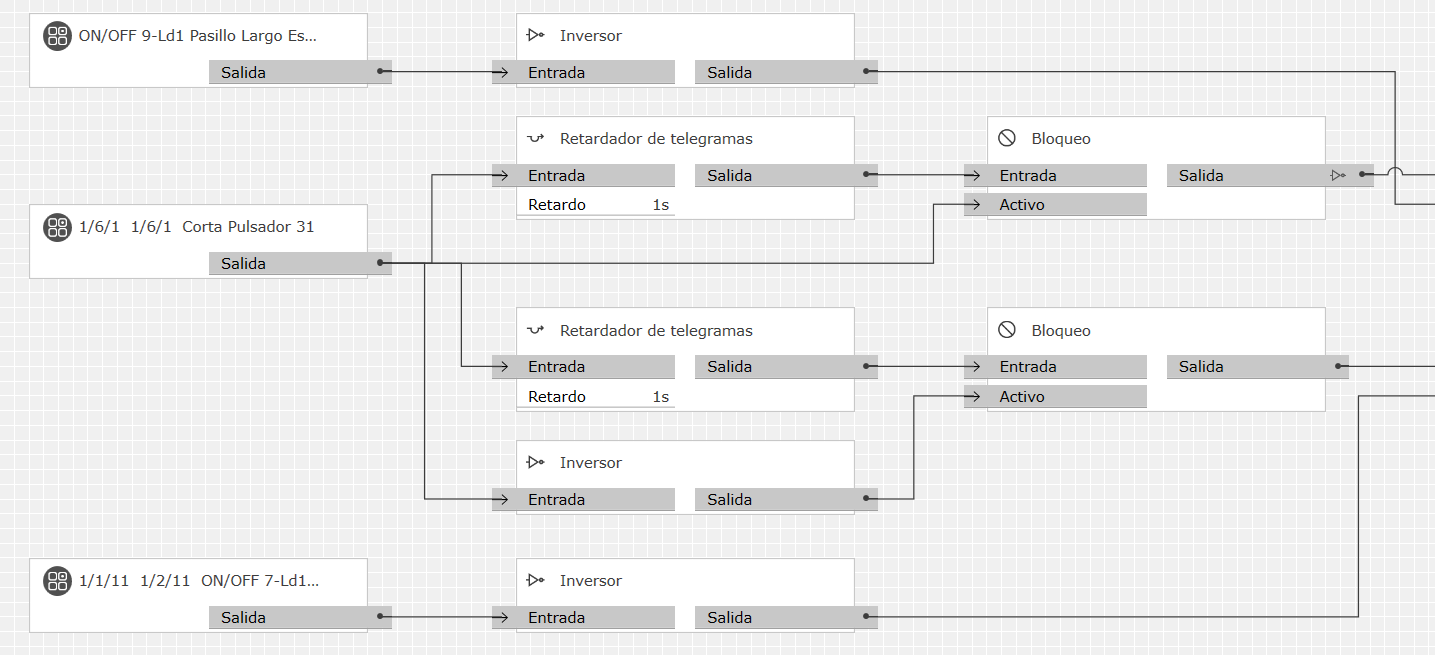
\includegraphics[width=1.15\textwidth]{figures/log_dimm_b21.png}  
\caption{Módulo lógico DIMMER: bloque 1 (v2)}
\label{fig:log_dimm_b21}
\end{figure}

Tanto la señal invertida del ON/OFF del estado de la lámpara como el valor de la salida del módulo “Bloqueo”, son dirigidos a un bloque “generador de valores”, respectivamente, a su puerto de “Valor” y al “Disparador” como se puede apreciar en la Imagen \ref{fig:log_dimm_b21}. 

\begin{figure}[H]
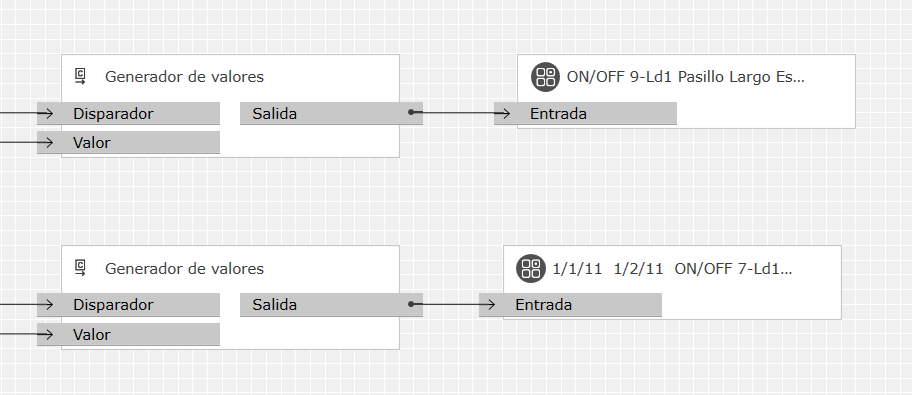
\includegraphics[width=0.95\textwidth]{figures/log_dimm_b22.png}  
\caption{Módulo lógico DIMMER: bloque 2 (v2)}
\label{fig:log_dimm_b22}
\end{figure}

Por lo tanto, uno de los dos módulos “Bloque” siempre enviará un pulso cuando la señal \textit{Corta Pulsador X} sea 0 y el otro cuando sea 1, provocando el disparo del “Generador de valores”, que enviará el valor invertido y contrario del valor de la señal ON/OFF. Este valor será conducido hasta un bloque “Salida” enlazado con la dirección de grupo del ON/OFF, que conmutará su valor, logrando por tanto cubrir con la pulsación corta de ambas teclas el control de esta variable.\\\\

El control de la regulación tendrá como entrada el valor recibido tras una pulsación larga sobre una de las teclas, y atacara siempre a la dirección de grupo \textit{Larga Pulsador X} con un valor de 12 ó -12. Esta señal es transmitida a dos bloques “Comparador”, enviando un 1 si reciben el valor adecuado. Cuando uno de estos bloques es activado y envía su señal, está ataca el puerto “Disparador” de un bloque “Generador de valores” con un valor de 10 fijado en su puerto “Valor”. \\
Por otro lado, es necesaria la creación de dos direcciones de grupo específicas, denominadas \textit{Estado X}, siendo X el código de la lámpara a controlar, e inicializadas con un valor inicial de 1 al arrancar el X1. La misión de esta variable interna del X1 es la de guardar el valor de la intensidad en una escala del 1 al 10. Tanto este valor acotado como el 10 enviado por el bloque “Generador de valores son enviados a un bloque “Multiplicación (x)”, siendo recibido el producto de ambas sobre un bloque “Salida” enlazado con la dirección de grupo del valor del dimmer. Esto permitirá regular la intensidad de la lámpara en saltos de 10 en 10 al ejecutar una pulsación larga sobre una de las teclas, al enviar ese valor como un dato de tipo porcentual a la luminaria.

\begin{figure}[H]
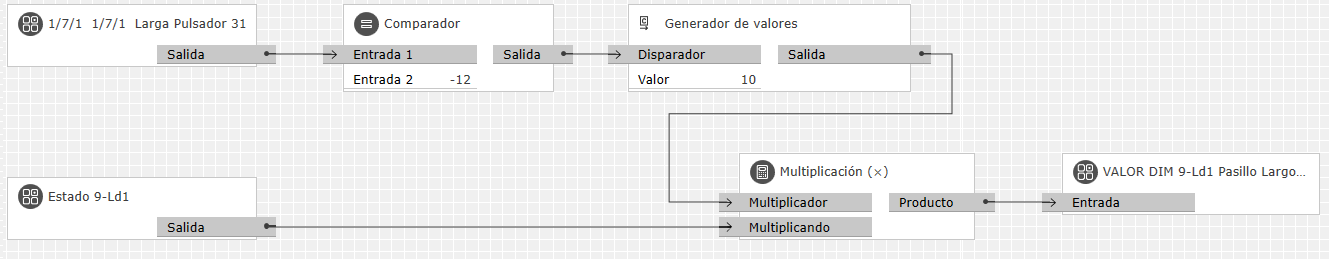
\includegraphics[width=1.15\textwidth]{figures/log_dimm_b23.png}  
\caption{Módulo lógico DIMMER: bloque 3 (v2)}
\label{fig:log_dimm_b23}
\end{figure}

Con la intención de evitar que el valor de la intensidad se salga de los límites impuestos de 10 y 100 y el sistema pueda entrar en algún tipo de conflicto o error, se ha diseñado una lógica que se encargará de corregir esta situación (Imagen \ref{fig:log_dimm_b24}). Contará con la señal \textit{Estado X} como entrada, atacando dos bloques comparadores: un “Mayor (>)” con un valor de 10 y otro “Menor (<)” con valor de 1 como números contra los que confrontarse. En el caso de que alguno de los dos bloques recibieran una señal que cumpliesen su premisa, enviaría un pulso a un bloque “Generador de valores” con el mismo valor, un 1 ó un 10 respectivamente, que sería enviado al bloque de salida direccionado a la propia dirección \textit{Estado X}. En las ocasiones que esto ocurriese, \textit{Estado X} actualizaría su valor y desencadenaría la ejecución de la rutina explicada anteriormente en la Imagen \ref{fig:log_dimm_b23}.

\begin{figure}[H]
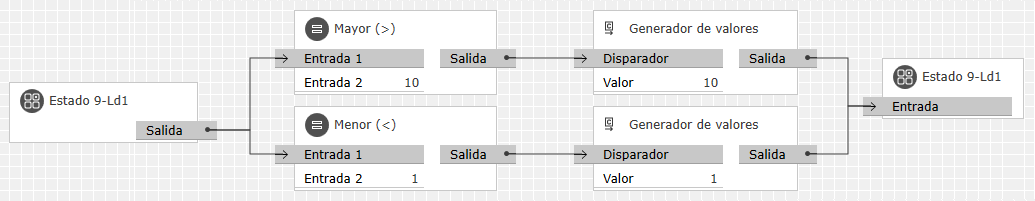
\includegraphics[width=1.15\textwidth]{figures/log_dimm_b24.png}  
\caption{Módulo lógico DIMMER: bloque 4 (v2)}
\label{fig:log_dimm_b24}
\end{figure}

Por último, se crea un bloque lógico para gestionar el control del valor de la propia variable \textit{Estado X}. Haciendo uso de la salida uno de los bloques “Comparador” de valor 12 ó -12, se activará un bloque “Luz de escalera”, cuyo propósito es mantener el envío de una señal tipo pulso durante un tiempo determinado. Debido a que los pulsadores han sido programados para enviar los telegramas en ciclos de 1 segundo, este bloque se ha programado para realizar el flanco de bajada una vez trascurridos 3 segundos desde su último activación, reiniciando la cuenta atrás cada vez que uno de los bloques “Comparador” lo dispara. Su puerto de salida se encuentra conectado a un bloque “Filtro” programado para no realizar ninguna acción al recibir un 1, pero al recibir un 0, deberá lanzar una señal que irá conmutando su valor de manera automática.  

\begin{figure}[H]
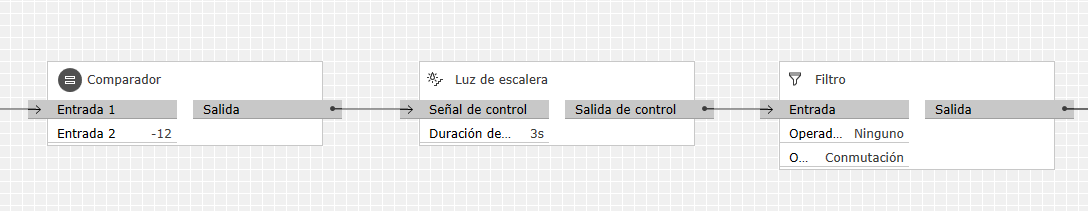
\includegraphics[width=1.15\textwidth]{figures/log_dimm_b25.png}  
\caption{Módulo lógico DIMMER: bloque 5 (v2)}
\label{fig:log_dimm_b25}
\end{figure}

Estos valores que conmutan irán conectados a dos bloques “Generadores de valores””: pasa por un bloque “Inversor” para llegar al que tiene en su puerto “Valor” un -1 y de manera directa al que tiene un valor de 1. Cuando alguno de estos bloques se activa, envía su valor a un tercer bloque “Generador de valores”, a su puerto “Valor” y será disparado por uno de los bloques “Comparador” con valor 12 ó -12 del inicio.

\begin{figure}[H]
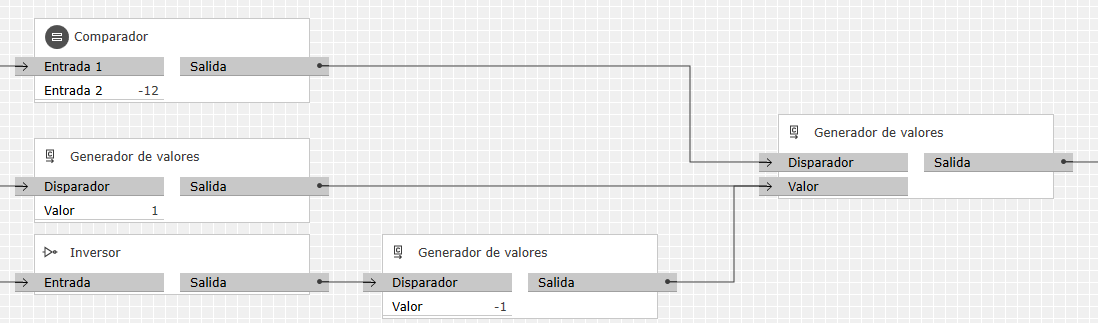
\includegraphics[width=1.15\textwidth]{figures/log_dimm_b26.png}  
\caption{Módulo lógico DIMMER: bloque 6 (v2)}
\label{fig:log_dimm_b26}
\end{figure}

Estos valores 1 y -1 son enviados alternativamente cada vez que termina la cuenta atrás de 3 segundos a uno de los puertos de entrada de un bloque “Operaciones aritméticas básicas” programado como sumador. El otro puerto de entrada será la salida de un bloque “Generador de valores” cuyo valor será el de \textit{Estado X} y será disparado, una vez más, por el bloque comparador de 12 ó -12. El resultado de la suma (o la resta en el caso de -1) de estos valores dará como resultado el valor que tomará la dirección de grupo \textit{Estado X}, actualizando su valor para la ejecución del próximo ciclo en el que se vea requerida.

\begin{figure}[H]
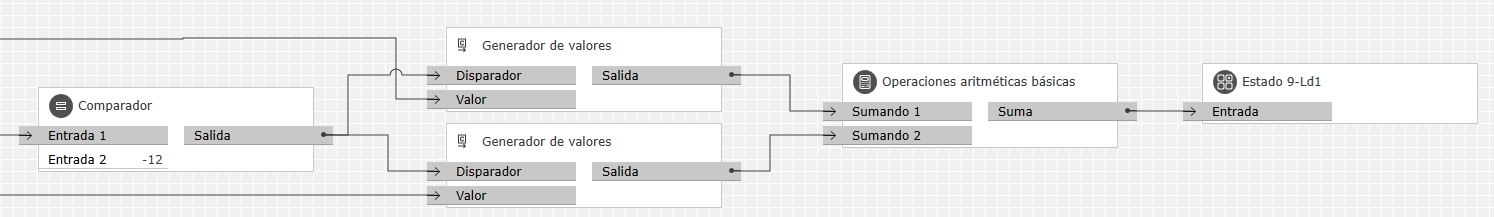
\includegraphics[width=1.15\textwidth]{figures/log_dimm_b27.png}  
\caption{Módulo lógico DIMMER: bloque 7 (v2)}
\label{fig:log_dimm_b27}
\end{figure}

A consecuencia del tiempo invertido en el diseño de esta mejora, aumentaron los costes relacionados con el personal, pero se logró obtener un resultado optimizado en cuanto a control, incluyendo la posibilidad de ser parametrizado a gusto del cliente de manera muy sencilla a través de la reprogramación de los tiempos de ejecución y envío de telegramas.

